\section{Introduction}

\subsection{Motivation}
\begin{frame}
	\frametitle{Introduction}
	\begin{itemize}
		\item Collecting images is easy\\
			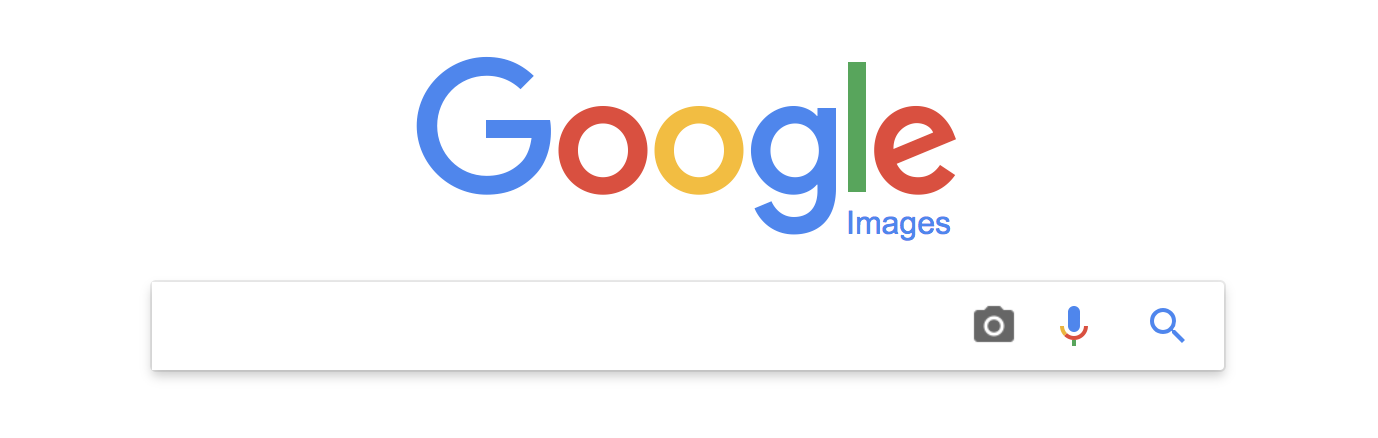
\includegraphics[scale=0.2, center]{images/google}
		\item Getting annotations for them is hard\\
			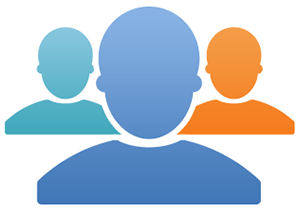
\includegraphics[scale=0.2, center]{images/amt}
		\item Need for algorithms that can utilize the unlabeled data
			\begin{itemize}
				\item Unsupervised - Representation Learning
				\item Weakly-supervised - Learning from coarse annotations
				\item Semi-supervised - Using both labeled and unlabeled data
			\end{itemize}
	\end{itemize}
\end{frame}

\subsection{Semi-Supervised Learning}
%\begin{frame}
%	\frametitle{Semi-Supervised Learning}
%	\begin{itemize}
%		\item Some labeled data available and the rest unlabeled
%		\item Use both to build better models
%	\end{itemize}
%\end{frame}

\begin{frame}
	\frametitle{Semi-Supervised Image Classification}
	\begin{itemize}
		\item Given two sets of images:
			\begin{itemize}
				\setlength\itemsep{0.5em}
				\item Labeled: $\mathcal{S} = \{(\mathbf{X}_i, y_i)\}_{i=1}^S$\\
				\item Unlabeled: $\mathcal{U} = \{\mathbf{X}_j\}_{j=S+1}^{S+U}$
			\end{itemize}
		\item Train an image classifier, $f(\mathbf{X};\Theta)$, which
			outputs a probability distribution, $\mathbf{q} = f(\mathbf{X}; \Theta)$, over classes $\mathcal{C}$
	\end{itemize}
\end{frame}

\subsection{Overview}
\begin{frame}
	\frametitle{Overview}
	\begin{itemize}
		\item We present unsupervised clustering and locality penalties
		\item Clustering encode knowledge about dataset class distribution
		\item Locality encodes the idea that objects occupy small regions
		\item No modifications to existing CNN architectures
		\item These can be used with cross-entropy for end-to-end training
	\end{itemize}
\end{frame}
